\scanpage{11}
\[
G''\supset H''\quad Q\quad H'\subset G'\quad P\quad G_k
\]
\[
\boxed{\begin{array}{l}
\alpha\in P(\mathbf C)\\
\beta\in Q(\mathbf C)\subset P'(\mathbf C)\\
\gamma\in P''(\mathbf C)
\end{array}}
\qquad
\begin{array}{l}
\beta\alpha=\gamma^{-1}\\
\gamma\beta=\alpha^{-1}\\
\alpha\gamma=\beta^{-1}
\end{array}
\]
\[
\left.\begin{array}{rl}
P&=\underline{\operatorname{Isom}}(T_B\otimes k,T_{DR})\\
Q\subset P'&=\underline{\operatorname{Isom}}(T_{DR},T_{Hdg})\simeq Q\mathbin{\times^{H'}}G'\\
P''&=\underline{\operatorname{Isom}}(T_{Hdg},T_B\otimes k)
\end{array}\right\}\text{déf}/k
\]
\diagram{\begin{tikzcd}
 & T_{Hdg}\otimes_k\mathbf C\arrow[dr,"\gamma"] & \\
T_{DR}\otimes_k\mathbf C\arrow[ur,"\beta"] & & T_B\otimes_{\mathbf Q}\mathbf C\arrow[ll,"\alpha"]
\end{tikzcd}}

\[
\left.\begin{array}{rl}
\mathrm{Fil}&=\underline{\operatorname{Filt}}_{\substack{\otimes,\ \text{dans}\ \deleted{\unsure{\xi}}\\\unsure{\text{classe int. de}|\text{classe ind. de}}\\\text{la filtration}\\\text{de }T_{DR}}}\ T_{\unsure{b|B}}\\[2em]
\mathrm{Big}&=\underline{\operatorname{Bigr}}_{\substack{\otimes,\ \text{dans}\\\unsure{\text{classe int. de}|\text{classe ind. de}}\\\text{la bigraduation}\\\text{de }T_{DR}}}\ T_B
\end{array}\right\}\text{déf}/\mathbf Q
\]

\margin{$U'\subset B'\subset G'$

$U':$ rad. unipotent de \unsure{$B'$}.

$B':$ parabolique associé à la filtration de $T_{DR}$.

$Q=$ fibré des sous groupes de Lévi de $B'$.
\diagram{\begin{tikzcd}
B'/U'\simeq L' & G_m\arrow[l,"j'"']
\end{tikzcd}}
hom central (\unsure{Tch})}

\margin{\figure{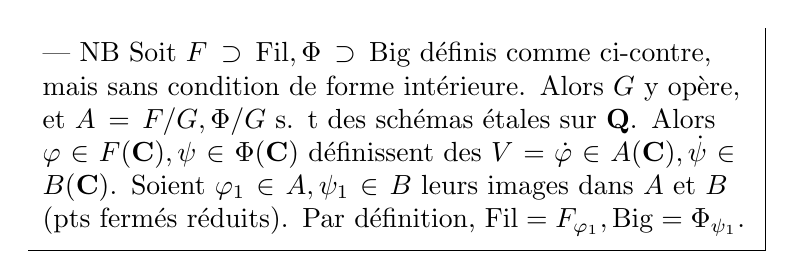
\begin{tikzpicture}
\node[align=left,text width=9cm,inner sep=5pt] (n) {--- NB Soit $F\supset\mathrm{Fil},\Phi\supset\mathrm{Big}$ définis comme ci-contre, mais sans condition de \unsure{forme intérieure}. Alors $G$ y opère, et $A=F/G,\Phi/G$ \unsure{s. t} des schémas \uline{\unsure{étales}} sur $\mathbf Q$. Alors $\varphi\in F(\mathbf C),\psi\in\Phi(\mathbf C)$ \deleted{définissent} des \unsure{$V=$} $\dot\varphi\in A(\mathbf C),\dot\psi\in B(\mathbf C)$. Soient $\varphi_1\in A,\psi_1\in B$ leurs images dans $A$ et $B$ (pts fermés réduits). Par définition, $\mathrm{Fil}=F_{\varphi_1},\mathrm{Big}=\Phi_{\psi_1}$.};
\draw (n.south west)--(n.south east)--(n.north east);
\end{tikzpicture}}}
\figure{\begin{tikzpicture}\draw[->] (0,0) .. controls (-.05,.3) and (-.2,.4) .. (-.55,.4);\end{tikzpicture}}

\margin{\uline{NB} Si on a $\varepsilon:\deleted{\unsure{G_m}}G'\longrightarrow G_m$ on a $(\varepsilon|B'/U')\circ j'=\mathrm{id}$. donc $j'$ mon. Si $H'\subset B'$ est l'image inverse de $\operatorname{Im}j'$ dans $B'$, alors \deleted{\unsure{le tout}} $j'$ est \inserted{donc} connu quand on connaît $H'$.}

\[
P\times P'\longrightarrow P'',\quad P'\times P''\longrightarrow P,\quad P''\times P\longrightarrow P',\qquad Q\subset P'
\]

\diagram{\begin{tikzcd}\mathrm{Big}\arrow[r,"p"] & \mathrm{Fil}\end{tikzcd}}
\deleted{\unsure{a}}
fibration, faisant de $B$ un torseur sur $\mathrm{Fil}$, de gr. $U_{\mathrm{Fil}}$, un groupe unipotent défini sur $F$, de dimension relative égale à $\dim U'$. $\mathrm{Fil}$ est de dim égale à $\dim G'/B'$, $\mathrm{Big}$ est de dim égale à $\dim G'/B'+\dim U'=\dim G'/L'$, \unsure{i.e.} $L'=\operatorname{Centr}(j'_0)$, $j'_0:G_{m_k}\longrightarrow H'$ relevant $j'$.

\margin{\figure{\begin{tikzpicture}
\node[draw,rounded corners=10pt,align=left,text width=8cm,inner sep=5pt] (a) {en fait, $\dot\varphi,\dot\psi$ sont dans $A(k),B(k)$ donc dans $A(k_1),B(k_1)$, où $k_1$ est la clôture alg. de $\mathbf Q$ dans $k$. D'ailleurs $F\longrightarrow\Phi$ induit $A\overset\sim\longrightarrow B$, donc};
\node[draw,align=left,text width=8cm,inner sep=5pt,anchor=north] at (a.south) {\unsure{autr. explicité en termes du groupe de Dynk. associé au réseau cor.} $\Gamma$ avec $W$ (Weyl) agissant : on \unsure{fera} $\Gamma/W$ par autom. extérieures....};
\end{tikzpicture}}}

On a un diagramme commutatif
\diagram{\begin{tikzcd}
P''\arrow[d,"\deleted{\unsure{q}}r"'] & P\arrow[d,"q"]\\
\mathrm{Big}_k\arrow[r,"p_k"'] & \mathrm{Fil}_k
\end{tikzcd}}
\[
\boxed{\begin{array}{l}\varphi=q(\alpha)\in\mathrm{Fil}(\mathbf C)\\\psi=r(\gamma)\in\mathrm{Big}(\mathbf C)\end{array}}
\qquad [\varphi=p(\psi)]
\]
\margin{$\dim G=g$\quad $\dim U'=u$\quad $\dim B'=b$\quad $\dim L'=\ell$\quad $(u+\ell=b)$}

\diagram{\begin{tikzcd}[row sep=small,column sep=small,execute at end picture={\draw ([xshift=-5pt,yshift=-5pt]current bounding box.south west) rectangle ([xshift=5pt,yshift=5pt]current bounding box.north east);}]
 & k(\alpha,\beta)=k(\beta,\gamma)=k(\gamma,\alpha)=K\arrow[dl,no head,"\leq u"']\arrow[dd,no head,"\leq u"]\arrow[ddr,no head,"\leq g"] & & \\
k(\gamma)\arrow[dd,no head,"\leq\ell"'] & & & \\
 & k(\alpha)\arrow[dd,no head,"\leq b"] & k(\beta)\arrow[ddd,no head,"\leq u"] & \\
k(\psi)\arrow[dr,no head,"\leq u" description]\arrow[dd,no head,"\mathrm{comp}"'] & & & \\
 & k(\varphi)\arrow[dr,no head,"\leq g-b" description]\arrow[dd,no head,"\mathrm{comp}"] & & \\
\mathbf Q(\psi)\arrow[dr,no head,"\leq u"'] & & k\arrow[dd,no head]\arrow[r,no head] & \substack{\mathbf Q(\varphi_1)\\\deleted{\unsure{\mathbf Q(\psi_1)}}=\mathbf Q(\varphi_1)}\\
 & \mathbf Q(\varphi)\arrow[dr,no head,"\leq g-b"] & & \\
 & \deleted{\unsure{\mathbf Q}} & \mathbf Q\arrow[uur,no head,"\mathrm{alg}"'] &
\end{tikzcd}}
\margin{\figure{\begin{tikzpicture}\node[draw,ellipse] {$\mathbf Q(\varphi_1)$ est \uline{indépendant}};\end{tikzpicture}} du plongement de $k$ dans $\mathbf C$, \unsure{donc} \illegible{3} \unsure{définit} \illegible{2} \unsure{du motif}.}
\[
\deleted{\unsure{K\subset k(\alpha)}}K\subset\deleted{\unsure{k(\alpha)}}\mathbf Q(k(\alpha),\overline{k(\alpha)})
\]
\[
(2i\pi)^n\in k(\alpha)\quad\text{si}\quad\mathbf Q(-n)\in\operatorname{Ob}\mathcal M
\]

\figure{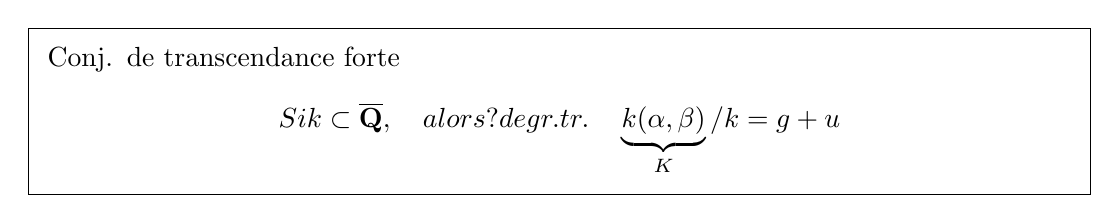
\begin{tikzpicture}
\node[draw,align=left,text width=13cm,inner sep=7pt] {
\uline{Conj. de transcendance forte}
\[
\text{Si } k\subset\overline{\mathbf Q},\quad\text{alors ? degr. tr.}\quad\underbrace{k(\alpha,\beta)}_K/k=g+u
\]
};
\end{tikzpicture}}
\[
\Longrightarrow\left\{\begin{array}{l}
\text{deg. tr.}\ k(\alpha)/k=g\\
\text{deg. tr.}\ k(\beta)/k=u\\
\text{deg tr.}\ k(\gamma)/k=g\\[.5em]
\text{deg. tr.}\ K/k(\beta)=g,\quad\text{et}\\
\text{deg tr.}\ K/k(\alpha)=\text{deg tr.}\ K/k(\gamma)=u\\[.5em]
\text{deg tr}\ \mathbf Q(\varphi)/\mathbf Q=g-b\\
\text{deg tr.}\ \mathbf Q(\psi)/\mathbf Q=g-b+u=g-\ell
\end{array}\right.
\]
\margin{10}
